\documentclass[aps,prl,twocolumn,showpacs,amsmath,amssymb,superscriptaddress]{revtex4-1}

\usepackage{graphicx}
\usepackage[justification=centerlast]{caption} % FIXME: 'justified' should be default, but it does not work
\usepackage{subfig}
\usepackage{amsbsy}
\usepackage{amssymb}
\usepackage{esint}
\usepackage{bm}
\usepackage[usenames]{color}

% FIXME: $\delta^{(D)}$ --- do we really need to specify dimension number? it can be deduced from the arguments. Same for $d^D$ in integrals.
% FIXME: it is better to avoid setting whole equations in bold --- we may need bold font for specific symbols (and I doubt that PRL style allows bold equations anyway)

\newcommand{\remark}[1]{\textcolor{red}{{[}#1{]}}}

\begin{document}

\title{ROUGH-DRAFT\_Quantitative simulations in three-dimensional atom interferometry}

\newcommand{\swinburneaffiliation}{ACQAO, Swinburne University of Technology, Hawthorn, VIC 3122, Australia}
\newcommand{\uqaffiliation}{ACQAO, Physics Department, University of Queensland, Queensland, Australia}

\author{B.~Opanchuk}
\affiliation{\swinburneaffiliation}
\author{M.~Egorov}
\affiliation{\swinburneaffiliation}
\author{S.~Hoffmann}
\affiliation{\uqaffiliation}
\author{A.~Sidorov}
\affiliation{\swinburneaffiliation}
\author{P.~D.~Drummond}
\affiliation{\swinburneaffiliation}

\begin{abstract}
We give a first-principles comparison of a calculation of quantum
phase-diffusion in a three-dimensional Bose gas,
as compared to recent experimental measurements.
Without using fitting parameters, we find excellent agreement
between the predicted fringe contrast and experimental data,
in an atom interferometer measurement.
\end{abstract}

\date{\today}

\maketitle

Atom interferometry is an important quantum technology,
at the heart of many suggested future applications of ultra-cold atomic physics.
Bose-Einstein condensates or atom lasers have potential advantages as detectors or sensors,
provided one can extract atomic phase information.
However, there is a challenge to be met.
Unlike photons, atoms can interact rather strongly, causing dephasing.
An intimate understanding of quantum many-body dynamics is essential in understanding
the precise nature of interaction-induced dephasing in the measurement process.
Progress in this technology therefore requires a quantitative theory of atom interferometry.

In this Letter we give a simple, yet quantitatively accurate
theoretical approach to calculations of atom interferometry at large atom number,
using a truncated Wigner representation.
This method extends the conventional Gross-Pitaevski equations
describing a Bose condensate to include quantum noise effects.
We show through comparison with experimental interferometric measurements on Bose condensates,
that the theory predicts observed dephasing results, within experimental errors.
No fitting parameters are required in these comparisons.
As a result, we suggest that the theoretical approach employed here
can be reliably used as a benchmark for predictions.
Importantly, we can clearly demonstrate where phase decay is driven by quantum fluctuations,
and where it is driven by trap inhomogeneity or other effects.

Quantum phase-diffusion is defined as the phase noise induced by number fluctuations,
which are intrinsically conjugate to phase.
As such, this is a fundamental limitation of any BEC interferometry,
and can only be removed when there are no interactions driving phase evolution.
However, there are other causes of density fluctuations as well as the overall number uncertainty,
which are also important in causing observed phase decays.
The important feature of the approach used here is that it is able to capture
all three significant features of atom interferometry that can result in decoherence.
These are:
\begin{itemize}
\item fluctuations caused by an atomic beam-splitter,
\item linear and nonlinear losses
\item trap inhomogeneity and propagation
\end{itemize}
We have not used variational or mean-field approximations.
Although these methods can certainly provide useful results,
they often require additional uncontrolled approximations.
Instead, the results given here simply require a controllable truncation
of an expansion in the inverse atom number.
They are applicable to simulations where the atom number per lattice point or mode is large.
Such quantitatively predictive theories have a great practical value
in assessing the utility of atom interferometry in new environments.
We expect that multi-configurational Hartree theories should give comparable or greater accuracy,
in principle, as they do not require truncation.
However, MCH methods are currently limited to lossless,
one-dimensional calculations with small atom numbers,
owing to computational complexity issues.

The theory we use is straightforward.
We start by assuming that the trapped BEC has S-wave interactions,
together with Markovian losses due to $n$-body collisions.
We employ the Wigner-Moyal quantum phase-space representation~\cite{Gardiner2004}
and the corresponding Lindblad-type master equation,
together with a truncation of third and higher-order derivatives in the equations of motion.
If we regard the commonly used Gross-Pitaevskii equation as a classical,
first approximation to mean-field condensate dynamics,
the truncated Wigner approach is best thought of as the second approximation
in an expansion in inverse particle number.
Such truncations have been shown to be valid in the limit of large particle number~\cite{Sinatra2002},
provided the effects of unoccupied vacuum modes can be neglected.
They are particularly useful in low-dimensional or trap environments,
where they have been succesful in predictions of quantum squeezing
and phase-diffusion effects to high accuracy in photonics~\cite{Corney2008}.
The truncation approximation has been further validated by comparison
with the exact positive-P method,
and with experiment in one-dimensional quantum soliton propagation dynamics.

In the present Letter, we treat an ultra-cold,
interacting multi-component spinor Bose gas in $D$ effective dimensions.
The basic Hamiltonian is easily expressed using quantum fields
$\widehat{\Psi}_{i}^{\dagger}({\mathbf{x}}),\widehat{\Psi}_{j}({\mathbf{x}})$,
where $\widehat{\Psi}_{i}^{\dagger}({\mathbf{x}})$ creates a bosonic atom of spin $i$
at location $\mathbf{x}$, and $\widehat{\Psi}_{i}({\mathbf{x}})$ destroys one;
the commutators are
$[\widehat{\Psi}_{i}(\mathbf{x}),\widehat{\Psi}_{j}^{\dagger}(\mathbf{x}')] =
\delta^{(D)}(\mathbf{x}-\mathbf{x}')\delta_{ij}\,\,.$
The resulting physics of a dilute, low-temperature Bose gas
is well-described in the S-wave scattering limit by an effective Hamiltonian
with contact interactions and external potentials:
	\remark{Is $\nabla \widehat{\Psi}_{i}^{\dagger} \cdot \nabla \widehat{\Psi}_{i}$
	equivalent to $\widehat{\Psi}_{i}^{\dagger} \nabla^2 \widehat{\Psi}_{i}$?}
	\remark{We can use the single integral sign and set of curly braces for all terms.}
	\remark{Do we need to explain how we performed the transition to local interaction?}
\begin{eqnarray}
	\widehat{H}/\hbar & = & \int d^{D}{\mathbf{x}} \left\{
		\frac{\hbar}{2m}{\nabla} \widehat{\Psi}_{i}^{\dagger} \cdot {\nabla} \widehat{\Psi}_{i} +
		\omega_{ij}(t,{\mathbf{x}}) \widehat{\Psi}_{i}^{\dagger} \widehat{\Psi}_{j}
	\right\} \nonumber \\
	& + & \int d^{D}{\mathbf{x}} \left\{
		\frac{g_{ij}}{2} \widehat{\Psi}_{i}^{\dagger} \widehat{\Psi}_{j}^{\dagger}
		\widehat{\Psi}_{j} \widehat{\Psi}_{i}
	\right\} \,\,.
\end{eqnarray}
Here we omit the field argument $({\mathbf{x}})$ for brevity,
and use the Einstein summation convention of summing over repeated indices.
Thus $\langle \widehat{\Psi}_{i}^{\dagger}({\mathbf{x}}) \widehat{\Psi}_{i}({\mathbf{x}}) \rangle$
is the spin $i$ atomic density, $m$ is the atomic mass,
and $g_{ij}$ is the atom-atom interaction term.
For a dilute gas at low enough temperatures,
$g_{ij}$ is related to the S-wave scattering length in three dimensions by:

\begin{equation}
	g_{ij}=\frac{4\pi\hbar^{2}a_{ij}}{m}.
\end{equation}
Here we implicitly assume a momentum cutoff $k_{c}=2\pi/\Delta z$,
where $\Delta z$ is a lattice cell-size which must be greater than the scattering length,
otherwise the couplings must be renormalized~\cite{Sinatra2002}.
	\remark{We made the transition to a discrete grid a bit too fast.}
	\remark{Moreover, cutoff mentioned here should not be confused with momentum cutoff
	introduced to avoid UV divergence~--- they can be different.}
The linear coupling term is given by:
\begin{equation}
	\omega_{ij}(t,{\mathbf{x}}) = \left[
		\omega_{i}+V_{i} \left( \mathbf{x} \right)
	\right] \delta_{ij} + \Omega_{ij}
\end{equation}
where $V_{i}$ is the external trapping potential for spin $i$,
$\omega_{i}$ is the internal Zeeman energy splitting associated with spin $i$,
and $\Omega_{ij}$ represents a time-dependent coupling
that is used to rotate one spin projection into another.

The truncated Wigner-Moyal quantum phase-space theory is well-suited
to these types of calculation of many-body dynamics.
The method employs a probabilistic (random) sampling of phase-space trajectories
to treat quantum fluctuations.
	\remark{We should mention that Wigner function is not exactly a probability distribution.}
This means that there are no complexity problems due to exponential growth
of the numbers of quantum states.
Furthermore, it is straightforward to treat a spatially inhomogeneous,
many-mode problem as found in an extended D-dimensional environment.
Initial conditions such as a coherent beam-splitter
as employed in typical atom interferometry experiments can be readily included.

This approach does require an approximation of truncating third-order derivatives
in an otherwise exact functional Fokker-Planck equation.
This approximation is valid at large atom number~\cite{Sinatra2002,Norrie2006},
where it has been checked in one-dimensional cases.
	\remark{Not exactly ``large atom number'', but ``number of atoms $\gg$ number of modes.''}
	\remark{It was checked in three-dimensional cases too, by Norrie.}
We note that in free-space calculations in three dimensions,
the ultra-violet (UV) divergence in free-space mode density at large momentum cutoff
makes the truncated Wigner method unreliable,
unless a momentum truncation is used so that each computed cell has atom number greater than unity.
	\remark{I would stick with $N \gg M$ condition.
	Cells near the borders will have 0 atoms regardless of the cutoff.}

In the relevant limits where the technique is applicable,
the equations simply reduce to Gross-Pitaevskii equations with Gaussian fluctuations
of the initial conditions and additional quantum noise \remark{or maybe ``stochastic?''} terms.
Damping and losses can be included via an additional Markovian master equation~\cite{Jack2002}
defined so that,
\begin{equation}
\bm{
	\frac{d\hat{\rho}}{dt} = -\frac{i}{\hbar} \left[ \hat{H}, \hat{\rho} \right] +
	\sum_{n,\mathbf{j}} \kappa_{\mathbf{j}}^{(n)}
	\int d^{3}\mathbf{r}\mathcal{L}_{\mathbf{j}}^{(n)} \left[ \hat{\rho} \right]
}
\end{equation}
	\remark{Shouldn't we use Einstein summation convention here too?}
	\remark{$n$ seems to be the number of interacting particles,
	and $j$ is the subtype (1--1, 1--2 and so on).
	Probably we should write that explicitly.}

Here we introduce local Liouville loss terms,
\begin{equation}
	\mathcal{L}_{\mathbf{j}}^{(n)} \left[ \hat{\rho}\right] =
	2 \hat{O}_{\mathbf{j}}^{(n)} \hat{\rho}\hat{O}_{\mathbf{j}}^{(n)\dagger} -
	\hat{O}_{\mathbf{j}}^{(n)\dagger}\hat{O}_{\mathbf{j}}^{(n)}\hat{\rho} -
	\hat{\rho}\hat{O}_{\mathbf{j}}^{(n)\dagger}\hat{O}_{\mathbf{j}}^{(n)}
\end{equation}
where the reservoir coupling operators $\hat{O}_{\mathbf{i}}^{(n)}$
are all $n$-fold products of local field annihilation operators,
\begin{equation}
	\hat{O}_{\mathbf{i}}^{(n)} =
	O_{\mathbf{i}}^{(n)} \left( \widehat{\boldsymbol{\Psi}} \right) =
	\widehat{\Psi}_{i_{1}} \left( \mathbf{r} \right)
	\widehat{\Psi}_{i_{2}} \left( \mathbf{r} \right) \ldots
	\widehat{\Psi}_{i_{n}} \left( \mathbf{r} \right)
\end{equation}
describing local $n$-body collision losses.
	\remark{Jack derives this form of loss operators only for 1--1--1 losses.}
Ignoring unitary evolution, the corresponding mean amplitude equations
for an $n$-body loss of this form are:
\begin{equation}
	\frac{\partial}{\partial t} \left\langle
		\widehat{\Psi}_{j} \left( \mathbf{r} \right)
	\right\rangle =
	-\left\langle \hat{\Gamma}_{j} \left( \mathbf{r} \right) \right\rangle
\end{equation}
	\remark{How was this derived?}
where we have introduced a nonlinear loss operator $\hat{\Gamma}_{j} \left( \mathbf{r} \right) =
\Gamma_{j} \left( \widehat{\boldsymbol{\Psi}} \left( \mathbf{r} \right) \right)$
as:
\begin{equation}
	\hat{\Gamma}_{j} \left( \mathbf{r} \right) \equiv
	\sum_{n,\mathbf{i}} \kappa_{\mathbf{i}}^{(n)}
	\frac{\partial\hat{O}_{\mathbf{i}}^{(n)\dagger}	\left( \mathbf{r} \right)}
		{\partial \hat{\Psi}_{j}^{\dagger} \left( \mathbf{r} \right)}
	\hat{O}_{\mathbf{i}}^{(n)} \left( \mathbf{r} \right) \,.
\end{equation}

As the full operator equations are highly nontrivial,
we proceed by using a stochastic phase-space method
that allows a numerical simulation of the condensate quantum dynamics~\cite{Drummond1993, Steel1998}.
Defining a Wigner function $W\left(\psi_{1},\psi_{2}\right)$,
where $\psi$ is a c-number field corresponing to the quantum field $\hat{\Psi}$,
this corresponds to a time-evolution equation of form:
\begin{equation}
	\frac{\partial W}{\partial t} = \int d\mathbf{r}\,\left\{
		-\frac{\delta}{\delta\psi_{i}} A_{i} +
		\frac{1}{2} \frac{\delta^{2}}{\delta\psi_{i} \delta\psi_{j}^{*}}D_{ij} +
		\mbox{O} \left[ \frac{\delta^{3}}{\delta\psi_{i}^{3}} \right]
	\right\} W
\end{equation}
	\remark{Should we mention functional Wigner correspondencies (Norrie)?}
	\remark{There are terms with order higher than 3 (up to $2n + 1$, to be precise).
	Moreover, the form $\delta\psi_{i}^{3}$ implies that all indexes in high-order terms
	are the same, which is not true.}
where higher derivative terms of type $\mbox{O}\left[\delta^{3}/\delta\psi_{i}^{3}\right]$
will be truncated.
This is equivalent to neglect of higher-order terms in an expansion in $1/\sqrt{N}$,
and is therefore valid in the limit of large particle number $N$.
	\remark{Again, probably it is better to use $N \gg M$ condition (Sinatra, Norrie).}
The drift term $A_{i}$ corresponds to Gross-Pitaevskii type evolution,
with additional nonlinear damping:
\begin{equation}
%\bm{ FIXME: bm and boldsymbol don't mix (latex just hangs)
	A_{i} = -\frac{i}{\hbar} \left(
	 	-\frac{\hbar^2}{2m} \nabla^{2} + g_{ij} \left| \psi_{j} \right|^{2}
	\right) \psi_{i} -
	\frac{i}{\hbar} \omega_{ij} \psi_{j} -
	\Gamma_{i} \left( \boldsymbol{\psi} \right)
%}
\end{equation}
	\remark{Changed form of the above equation~---
	I think it is better to make it look like $-i/\hbar H$, and use SI everywhere.}
	\remark{$\Gamma_{i}$ here is a classical loss term,
	not to be confused with $\hat{\Gamma}_{i}$.}

The next highest order term in the evolution equation gives rise to
quantum noise associated with the loss reservoirs,
with:
\begin{equation}
	D_{ij} = \sum_{n,\mathbf{k}} \kappa_{\mathbf{i}}^{(n)}
	\frac{\partial O_{\mathbf{k}}^{(n)*}}{\partial\psi_{i}^{*}}
	\frac{\partial O_{\mathbf{k}}^{(n)}}{\partial\psi_{j}}
\end{equation}
	\remark{Again, what is the connection between $O$ and $\hat{O}$?}
	\remark{There are additional terms: any combination of partial derivatives
	$\partial/\partial\psi_{i}$, $\partial/\partial\psi_{i}^*$.}

With the inclusion of reservoir couplings to describe losses
the truncated Fokker-Planck equation can be transformed
to a coupled stochastic Gross-Pitaevskii equation:
\begin{equation}
	\frac{d\psi_{j}}{dt} = iK_{j} \psi_{j} - ig_{ij} |\psi_{i}|^{2} \psi_{j} - \Gamma_{j} +
		\sum_{n,\mathbf{i}} \gamma_{\mathbf{i},j}^{(n)} \zeta_{\mathbf{i}}^{(n)} (\mathbf{x},t)
\end{equation}

Here the linear unitary evolution of the wave-function, is described by:
\begin{equation}
	K_{j} = \hbar \nabla^{2}/2m - \omega_{j} - V_{j} \left( \mathbf{r} \right)
\end{equation}
while $\zeta_{\mathbf{i}}^{(n)}(t,\mathbf{x})$ is a complex,
stochastic delta-correlated Gaussian noise with
\begin{equation}
	\left\langle
		\zeta_{\mathbf{i}}^{(n)} (\mathbf{x},t) \zeta_{\mathbf{j}}^{(m)}(\mathbf{x}',t')
	\right\rangle =
	\delta_{\mathbf{ij}} \delta^{nm} \delta^{D} \left(
		\mathbf{x} - \mathbf{x}'
	\right)
	\delta \left( t - t' \right)\,.
\end{equation}
The multiplicative noise coefficient~---
\begin{equation}
	\gamma_{\mathbf{i},j}^{(n)} \left( \boldsymbol{\psi} \right) =
	\sqrt{\kappa_{\mathbf{i}}^{(n)}}
	\frac{\partial O_{\mathbf{k}}^{(n)}}{\partial\psi_{j}}
\end{equation}
is needed as a fluctuation-dissipation term,
to ensure that the losses do not remove the vacuum fluctuations,
so that the Wigner variables remain equivalent to the corresponding operators.
	\remark{Looks too easy. How did we make the transition from FPE to this
	without decomposing the diffusion matrix?}

For initial conditions in interferometry it is usually sufficient
to consider a coherent state amplitude $\Psi_{s}^{c}$,
corresponding to a typical initial state with Poissonian number fluctuations.
In this case the initial Wigner amplitude has a Gaussian random distribution,
with $\Psi_{s}(\mathbf{x},t_{0})=\Psi_{s}^{c}(\mathbf{x})+\Delta\Psi_{s}(\mathbf{x})$,
where:
\begin{equation}
	\left\langle
		\Delta\Psi_{s}(\mathbf{x}) \Delta\Psi_{u}^{*}(\mathbf{x}')
	\right\rangle =
	\frac{1}{2} \delta_{su} \delta^{D} \left( \mathbf{x} - \mathbf{x}'\right)
\end{equation}
For greater accuracy, the coherent-state initial condition
can be modified to account for initial ground-state correlations,
or additional number-fluctuations above the Poissonian level.
The Wigner representation generates symmetrically ordered correlation functions.
In numerical simulations, the delta-function correlations are simply replaced by
local correlations at each lattice point,
with a variance of $1/\Delta V$, where $\Delta V$ is the lattice cell volume.
	\remark{In fact, I am now adding vacuum particles in k-space --- it is easier.}
If a normal ordered correlation is measured~--- typical of an absorption image~---
one must calculate the measured atomic densities according to
$n_{s} \left( \mathbf{x} \right) = \left\langle
	\Psi_{s}(\mathbf{x}) \Psi_{s}^{*}(\mathbf{x})
\right\rangle -1/2\Delta V$,
to correct for vacuum fluctuations.
	\remark{Again, we have to mention that $W$ is not exactly a probability distribution.}
In practical terms, truncation errors start to become significant
when the number of particles per cell is of order unity or less.

As a specific example of the utility of this method,
we consider recent three-dimensional dipole trap interference experiments,
involving ground-states of $\textrm{Rb}^{87}$ with quantum numbers $F=1,\, m_{F}=+1$
and $F=2,\, m_{F}=-1$ respectively.

\def\imagetop#1{\vtop{\null\hbox{#1}}}

\begin{figure}
	\begin{tabular}{l l}
	\imagetop{\hspace*{0.381in}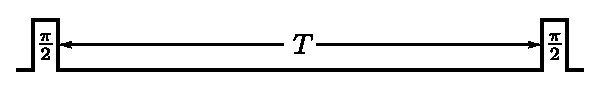
\includegraphics[width=1.95in]{figures/ramsey_sequence.eps}} & \imagetop{(a)} \\
	\imagetop{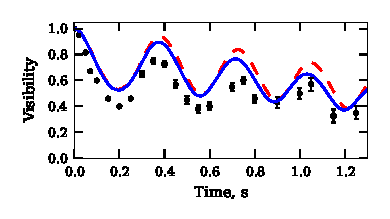
\includegraphics{figures/ramsey_visibility.eps}} & \imagetop{(b)} \\
%	\vskip 0.2cm
	\imagetop{\hspace*{0.381in}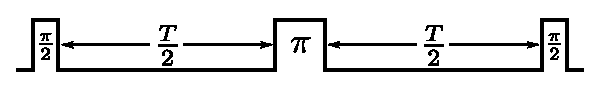
\includegraphics[width=1.95in]{figures/echo_sequence.eps}} & \imagetop{(c)} \\
	\imagetop{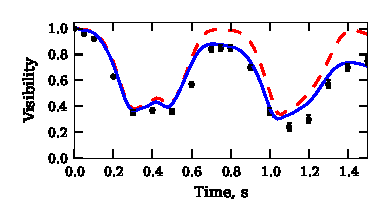
\includegraphics{figures/echo_visibility.eps}} & \imagetop{(d)}
	\end{tabular}

	\caption{(color online).
	Schematic of interferometric sequence for Ramsey (a) and Ramsey with symmetric spin-echo (c),
	(b) and (d) are the corresponding plots of visibility $A$,
	measured in the phase domain as a function of evolution time T.
	Experimental data points (filled circles) agree well with simulations
	when the effects of classical and quantum noise are added (black solid line),
	to the coupled GPE theory (red dotted line).
	Blue dashed line represent the effect of only quantum noise.}

	\label{fig:visibility}
\end{figure}

\begin{figure}
	\begin{tabular}{l l}
	\imagetop{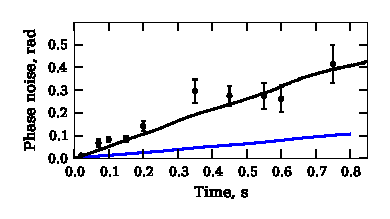
\includegraphics{figures/ramsey_phnoise.eps}} & \imagetop{(a)} \\
	%	\vskip 0.2cm
	\imagetop{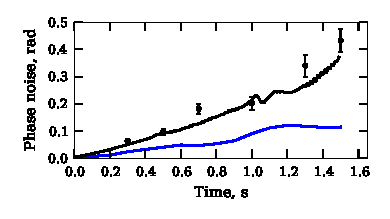
\includegraphics{figures/echo_phnoise.eps}} & \imagetop{(b)}
	\end{tabular}

	\caption{(color online).
	Schematic of interferometric sequence for Ramsey (a) and Ramsey with symmetric spin-echo (c),
	(b) and (d) are the corresponding plots of visibility $A$,
	measured in the phase domain as a function of evolution time T.
	Experimental data points (filled circles) agree well with simulations
	when the effects of classical and quantum noise are added (black solid line),
	to the coupled GPE theory (red dotted line).
	Blue dashed line represent the effect of only quantum noise.}

	\label{fig:phasenoise}
\end{figure}


\bibliography{qsim}

\end{document}
